% Тут используется класс, установленный на сервере Papeeria. На случай, если
% текст понадобится редактировать где-то в другом месте, рядом лежит файл matmex-diploma-custom.cls
% который в момент своего создания был идентичен классу, установленному на сервере.
% Для того, чтобы им воспользоваться, замените matmex-diploma на matmex-diploma-custom
% Если вы работаете исключительно в Papeeria то мы настоятельно рекомендуем пользоваться
% классом matmex-diploma, поскольку он будет автоматически обновляться по мере внесения корректив
%

% По умолчанию используется шрифт 14 размера. Если нужен 12-й шрифт, уберите опцию [14pt]
\documentclass[14pt]{matmex-diploma}
%\usepackage{float}          % необходимо для указания места картинки на странице
%\documentclass{matmex-diploma}


\usepackage{mathtools}      % матрицы 
\usepackage{amsfonts}
\usepackage{multicol,caption,float, subfig} % картинки

\hyphenpenalty=10000    % пенальти на переносы (max)
\sloppy % режим разрешает разрежать строки
\widowpenalty=4000 % пенальти на висячие строки в конце абзаца  
\clubpenalty=4000 % пенальти на висячие строки в начале абзаца


\begin{document}
% Год, город, название университета и факультета предопределены,
% но можно и поменять.
% Если англоязычная титульная страница не нужна, то ее можно просто удалить.
\filltitle{ru}{
    faculty = {Математическое обеспечение и администрирование информационных систем},
    chair              = {Информационно-аналитические системы},
    title              = {Рекомендательная система для образовательного контента},
    % Здесь указывается тип работы. Возможные значения:
    %   coursework - Курсовая работа
    %   diploma - Диплом специалиста
    %   master - Диплом магистра
    %   bachelor - Диплом бакалавра
    type               = {bachelor},
    position           = {студента},
    group              = 441,
    author             = {Волжина Елена Григорьевна},
    supervisorPosition = {ст. преп.},
    supervisor         = {Ярыгина А.\,С.},
%    reviewerPosition   = {ст. преп.},
    reviewer           = {Вяххи Н.\,И.},
    chairHeadPosition  = {профессор},
    chairHead          = {Новиков Б.\,А.},
    university         = {Санкт-Петербургский Государственный Университет},
    city               = {Санкт-Петербург},
    year               = {2016}
}
\filltitle{en}{
    faculty = {Software and Administration of Information Systems},
    chair              = {Analytical Information Systems},
    title              = {Recommender system for educational content},
    type               = {bachelor},
    author             = {Elena Volzhina},
    supervisorPosition = {senior assistant prof.},
    supervisor         = {Anna Yarygina },
%    reviewerPosition   = {assistant},
    reviewer           = {Nikolay Vyahhi},
    chairHeadPosition  = {professor},
    chairHead          = {Boris Novikov},
    year               = {2016}
}
% TODO: разобраться с порядком в bib

\maketitle
\tableofcontents


% У введения нет номера главы
\section*{Введение}
В современном мире онлайн-образование постепенно становится все более популярным. Возможность учиться у профессоров ведущих учебных заведений, изучать новые области, получать нужные в работе знания, не выходя из дома, привлекает большое количество людей. 
\\\indent Одной из наиболее распространенных форм онлайн-обучения являются массовые открытые онлайн-курсы (MOOC, massive open online course). Чаще всего они включают видео, слайды и текстовый контент, подготовленные преподавателем, а также задачи для проверки знаний, которые обычно проверяются автоматически, но также возможна проверка студентами работ своих товарищей. В качестве задач могут быть предложены самые разнообразные типы заданий: от простого выбора правильного ответа до задач на программирование и написания эссе.
\\\indent У онлайн-образования есть свои особенности, отличающие его от обычного, офлайн-образования. Среди плюсов, во-первых, уже упомянутая выше доступность каждому, у кого есть доступ к интернету. Во-вторых, это почти неограниченная масштабируемость: благодаря автоматизированной проверке задач на курсе могут одновременно учиться тысячи человек, что несопоставимо с обычными курсами в учебных аудиториях. В-третьих, каждый студент может выбирать удобное для себя время и темп для прохождения материала. В-четвертых, в распоряжении преподавателей оказывается большое число данных о том, как пользователи проходят его курсы, которые он может использовать для анализа и улучшения своих материалов.
\\\indent В то же время в онлайн-обучении есть и минусы. В отличие от традиционного образования, где у студента всегда есть мотивация в виде оценки его академической успеваемости, в случае онлайн-курсов нет никаких штрафов за не пройденный курс. Из-за этого доля закончивших курс из записавшихся на него редко превышает $10\%$. Помимо этого, из-за большого числа учащихся у преподавателя нет никакой возможности уделять индивидуальное внимание каждому студенту сообразно его уровню и возможностям.
\\\indent В таблице \ref{tabular:mooc_statistic} представлены сведения о нескольких популярных платформах для онлайн-курсов. Последняя из них, \textit{stepic.org}, содержит в основном материалы на русском языке. В рамках этой работы была разработана и исследована рекомендательная система для этого сайта.

\begin{table}[t]
    \caption{Платформы с онлайн-курсами}
    \label{tabular:mooc_statistic}
    \begin{center}
    \begin{tabular}{c|c|c}
    \hline
    Название & Год запуска & Пользователей \\
    \hline
    \hline
    Coursera\cite{coursera} & 2012 & 15 млн \\
    edX\cite{edx} & 2012 & 5 млн \\
    Udacity\cite{udacity} & 2012 & 1.6 млн \\
    Stepic.org\cite{stepic} & 2013 & 180 тыс. \\
    \hline
    \end{tabular}
    \end{center}
\end{table}

\indent Задача этой работы -- создать рекомендательную систему, которая могла бы посоветовать студенту контент, который будет интересен ему, и которая также будет учитывать уровень подготовки студента, его знания и пробелы. Кроме этого система должна уметь оценивать сложность контента. Это нужно, в частности, для адаптивных рекомендаций, которые будут помогать пользователю изучать материал, гибко подстраиваясь под него, предлагая именно тот контент, который ему нужен сейчас для обучения.
\\\indent Такая система будет полезна пользователям персонализованными рекомендациями, которые могут помочь им изучить конкретную тему или предложить что-то новое.
%TODO: тут тоже стоит еще дополнить про адаптивное обучение, когда будет больше информации, также вообще про полезность рекомендательной системы


\section{Существующие{\kern 0.5em}рекомендательные системы}

\indent Тема рекомендательных систем активно исследуется последние десятилетия\cite{goldberg1992using}\cite{Mahmood}\cite{Anand}. Она широко применима на практике, в том числе в коммерции, что значительно стимулирует ее развитие, как в плане теоретических исследований, так и в виде практических задач. 
\\\indent В качестве одного из первых примеров рекомендательной системы в современном представлении можно привести \textit{movielens.org}\cite{movielens}, предлагающий пользователям фильмы на основе их предпочтений. Этот сервис интересен тем, что он предоставляет всем желающим обширный набор данных о фильмах и рейтингах, поставленных им пользователями. Этот набор данных был использован в большом числе исследований в области рекомендательных систем последних двух десятилетий.  
\\\indent Существует два основных класса рекомендательных систем\cite{rec_sys_handbook}:
\begin{itemize}
    \item Системы, основанные на \textit{фильтрации контента}. Такие системы предлагают пользователям контент, похожий на тот, что они изучали ранее. Схожесть подсчитывается с помощью характеристик сравниваемых объектов. Например, для рекомендации фильмов можно использовать близость жанров или актерский состав. Такой подход используется в сервисе для оценки, поиска и рекомендаций фильмов \textit{Internet Movie Database}\cite{imdb}.
    \item Системы, использующие \textit{коллаборативную фильтрацию}. В этом случае пользователю предлагается контент, заинтересовавший похожих на него пользователей. Рекомендации сервиса MovieLens основаны именно на этом подходе.
    \item \textit{Гибридные} системы, комбинирующие два предыдущих подхода. Система такого типа используется в  \textit{Netflix}\cite{netflix}, сервисе для онлайн-просмотра фильмов и сериалов.
\end{itemize}

\indent В данной работе будет создана гибридная система с более активным использованием фильтрации контента и менее активным -- коллаборативной фильтрации.

\\\indent Существует множество исследований, посвященных рекомендательным системам для обучения, основанного на использовании технологий (\textit{Technology Enhanced
Learning})\cite{rec_sys_handbook:tel}. Специфика задачи в этом случае добавляет новые направления развития рекомендательной системы. Во-первых, это возможность построения адаптивной рекомендательной системы, которая будет подстраиваться под нужды пользователя в конкретный момент и предлагать ему оптимальные пути изучения материала\cite{adaptive}. В таком формате могут быть реализованы различные тренажеры, например, по математике или какому-либо языку программирования, содержащие набор задач разной сложности, из которых разным ученикам будут в каждый момент времени подходить разные. Во-вторых, можно извлечь зависимости между обучающими материалами из данных о том, как пользователи их проходят. Эти данные могут помочь выделить отдельные темы в материалах, связи между этими темами, их соотношения по сложности\cite{learning_networks}.

\\\indent Упомянутые ранее платформы для онлайн-обучения используют свои рекомендательные системы, советуя пользователям курсы, которые их могут заинтересовать. Недостаток этих рекомендаций в том, что они могут предложить только курс целиком, но не какую-то его часть, даже если пользователю будет интересна только она. Также построенная таким образом система никак не может помочь пользователю в изучении курса, который он выбрал.
\\\indent Рекомендательная система ресурса MathsGarden\cite{mathsgarden} работает, напротив, с самыми небольшими частями контента -- отдельными задачами. Она представляет собой тренажер по элементарной арифметике для учеников начальной школы, который предлагает ученику задачи, оптимально подходящие ему в данный момент времени по сложности. Для этого система подсчитывает и динамически изменяет относительную характеристику знаний ученика, а также характеристику сложности задач. Эта система будет подробно рассмотрена позже.


\section{Платформа stepic.org}
\indent Платформа \textit{stepic.org}\cite{stepic} -- сайт с большой русскоязычной аудиторией, на котором размещено несколько десятков онлайн-курсов, преимущественно технической тематики. Каждый из них прошли от нескольких сотен до нескольких тысяч человек. Ежедневно на платформу заходят тысячи учащихся. Это крупнейший в России ресурс для онлайн-образования.
\subsection{Терминология}
\indent Курсы на stepic.org разделены на \textit{модули}, каждый модуль обычно рассчитан на неделю или две. У модуля могут быть установлены дедлайны на решение задач. После жесткого дедлайна пользователь все еще может проходить модуль, но уже не получит баллов за решение задач. Еще у модуля может быть мягкий дедлайн, после которого пользователь получит за решение задач часть баллов.
\\\indent Модуль состоит из \textit{уроков}, каждый из которых посвящен отдельной небольшой теме. Обычно уроки формируются так, чтобы можно было рассматривать урок в отрыве от курса, то есть как отдельную структурную единицу.
\\\indent На рис.~\ref{fig:course} можно увидеть пример структуры курса, состоящего из трех модулей.

\begin{figure}[t]
\centering
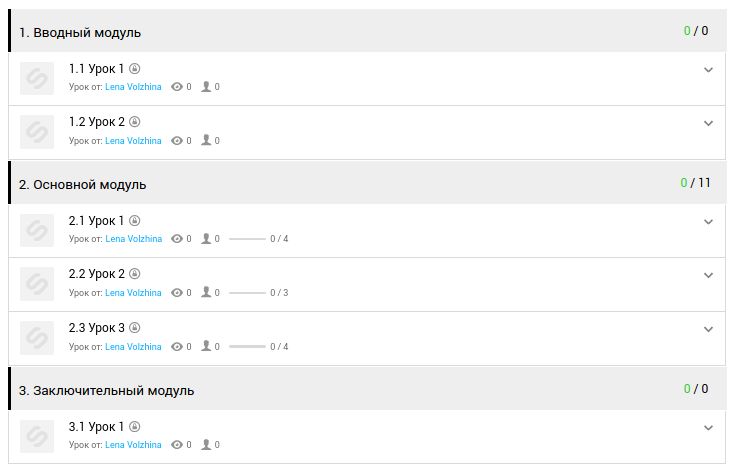
\includegraphics[width=\linewidth]{images/course_structure.png}
\caption{Структура курса}
\label{fig:course}
\end{figure}

\\\indent В каждом уроке есть несколько \textit{шагов} (\textit{стэпов}), представляющих собой либо лекционный материал в виде видеозаписи или текста, либо задачу одного из множества видов. Бывают задачи-тесты с выбором ответа, задачи с текстовым ответом, задачи на программирование и многие другие. Большинство из них предполагают моментальную автоматическую проверку системой, но есть также задачи на написание эссе, которые студенты сами проверяют друг у друга на основе сформулированных преподавателем критериев.
% вода: типы задач, возможности проведения хакатонов или еще чего
\\\indent Каждый урок или курс может быть помечен \textit{тегом} -- концепцией, которая описывает его содержимое. Примеры таких тегов: программирование, linux, статистика. Каждый тег привязан к объекту в базе знаний Wikidata\cite{wikidata}.
\\\indent Уроки могут быть объединены в \textit{пути}. В отличие от курсов, у путей нет модулей, дедлайнов и возможности получить сертификат за их прохождение. Это просто способ объединять уроки в логическую последовательность. Обычно после того, как курс закрывается для просмотра, его уроки собираются в путь и выкладываются в библиотеку.



\subsection{Возможности}
\indent В основном студенты приходят на stepic.org, чтобы изучать курсы. Успешно прошедшие курс и набравшие нужное количество баллов получают электронные сертификаты. Преподаватели могут установить границу для получения обычного сертификата, и для получения сертификата с отличием.
\\\indent Помимо курсов на stepic.org также есть раздел уроков. Уроки, которые были включены в один курс, здесь располагаются без связи друг с другом. 
\\\indent Stepic.org позволяет пользователям создавать свои уроки и курсы, давать ссылки на них или же встраивать в другие сайты. Также имеется возможность интеграции с любой платформой через LTI, благодаря чему в некоторых курсах на платформе Coursera\cite{coursera} используются задачи, которые создаются и проверяются на stepic.org. Весь контент на платформе распространяется под открытой лицензией Creative Commons\cite{creativecommons}.
\\\indent Пользователи могут общаться между собой с помощью комментариев под каждым шагом. Там обычно обсуждают лекционный материал, помогают в решении задач или общаются с преподавателями.
\\\indent Для удобства обучения на платформе разработана рекомендательная система, описанная в этой работе. Она помогает пользователям находить интересные им материалы.


\section{Реализация рекомендательной системы}
\indent В рамках данной работы была реализована рекомендательная система, которая предлагает пользователю новые уроки на основании того, чем он интересовался ранее. Она использует для этого различные способы найти контент, чем-то похожий на тот, который пользователь уже изучал, или же не столь похожий, но в целом интересный. Каждый из таких способов оформлен в виде отдельной функции (\textit{хендлера}), которая извлекает список уроков по заложенному в нее принципу и размечает их весами в зависимости от того, насколько они подходят пользователю. Подробное описание этих функций-хендлеров будет представлено ниже.
\\\indent Рекомендательная система может применяться в разных ситуациях. Два основных случая:
\begin{itemize}
    \item просто рекомендация для конкретного пользователя, которая показывается ему на главной странице и во вкладке <<Рекомендованные уроки>>, а также время от времени присылается на почту;
    \item \textit{контекстная} рекомендация, которая показывается пользователю после прохождения урока вне курса (то есть урока, для которого нет фиксированного следующего за ним), как подсказка, что посмотреть дальше.
\end{itemize}

\indent Вместе с рекомендацией пользователю также показывается информация о том, почему ему был предложен именно этот урок. Эту информацию легко извлечь благодаря тому, что в каждую функцию-хендлер заложена какая-то естественная интуиция, так что можно восстановить причину рекомендации.
\subsection{Информация о пользователе}
В процессе обучения на stepic.org пользователь оставляет значительный цифровой след. Помимо информации о его прогрессе сохраняются также сведения о том, когда он посещал разные шаги, когда пытался решать задачи и с каким результатом, и даже как он смотрел видео: какие установил скорость и громкость, где останавливал и где перематывал. 
\\\indent Наиболее интересны для базовой рекомендательной системы следующие сведения: теги, которыми пользователь интересовался, уроки, на которые он заходил, уроки, которые он прошел, а также, если рекомендация контекстная, текущий урок.
\\\indent Кроме информации о конкретном пользователе, сохраненные данные можно рассматривать как сведения о взаимодействии пользователей с контентом. Одним из способов аггрегировать и использовать эти сведения являются графы переходов, о которых подробно рассказано в следующем параграфе.


\subsection{Графы переходов}
\indent Часто бывает полезно узнать, как пользователи изучают контент, что они смотрят чаще, что реже, какие материалы проскакивают, на какие возвращаются, и, что немаловажно, в каком порядке их смотрят. Используя сохраненные данные о действиях пользователей, несложно дать ответы на эти вопросы. Для этого был использован \textit{граф переходов} (\textit{process map}), то есть такой ориентированный граф, в котором вершинами будут единицы контента (например, шаги или уроки), а веса дуг будут показывать количество переходов между этими единицами контента.
\\\indent Многим действиям, которые совершают пользователи на платформе, соответствуют записи в таблице \textit{событий}. У каждого события есть временная метка, что позволяет расположить события на временной шкале. События разделены на типы, соответствующие действиям пользователя, например, <<viewed>> (открыл шаг), <<succeeded attempt>> (решил задачу) или <<commented>> (оставил комментарий). Нас будут интересовать действия пользователя по отношению к шагам, которые затем легко обобщить на уроки, к которым эти шаги принадлежат, и даже на теги, которыми уроки помечены.
\\\indent Визуально граф переходов можно представить себе как ряд вершин-материалов (например, шагов), между некоторыми из которых есть дуги. Наличие дуги между двумя шагами означает, что существуют пользователи, которые просмотрели их друг за другом. Каждая дуга обладает меткой, содержащей число таких пользователей. Пример графа переходов для шагов одного урока внутри курса можно увидеть на рис.~\ref{fig:process_map_example}.

\begin{figure}[t]
\centering
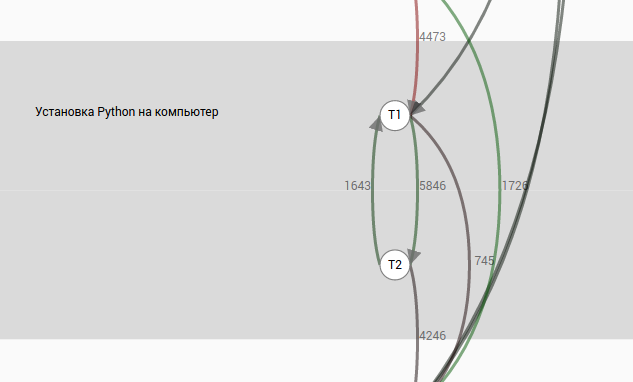
\includegraphics[width=0.65\linewidth]{images/process_map_example.png}
\caption{Граф переходов для шагов одного урока}
\label{fig:process_map_example}
\end{figure}

\indent Процесс построения графа переходов тривиален: для каждого пользователя мы рассматриваем все его действия по отношению к шагам, сортируем их по времени, и затем подсчитываем для каждой пары шагов, сколько раз он совершал действие с одним из них непосредственно после действия с другим. Далее эти частоты суммируются для всех пользователей, и получается общий граф переходов.
\\\indent Изначально графы переходов по шагам использовались, чтобы преподаватели могли изучить статистику по своим курсам, посмотреть, в каком порядке пользователи смотрят материалы, где есть странные переходы. Для простоты анализа по курсу вычислялась средняя частота перехода между шагами (с учетом того, теория в шаге или задача, а также с учетом положения шага в уроке), и ребра в итоговом графе окрашивались зеленым, если переход по ним происходил чаще ожидаемого, или красным, если реже. Фрагмент графа переходов по одному из курсов представлен на рис.~\ref{fig:processmap}. По этому фрагменту видно, что шаг с теорией Т4 чаще обычного пропускают и переходят к следующему за ним.
\\\indent Далее графы переходов стали строиться не только по шагам, но также по урокам и тегам, чтобы использовать это в рекомендательной системе. Граф переходов по урокам строится по тому же принципу, что и для шагов, просто действия над шагами рассматриваются как действия над уроками, к которым эти шаги принадлежат. Для тегов процесс аналогичен: действия со шагами переводятся в действия с тегами их уроков.


\begin{figure}[t]
\centering
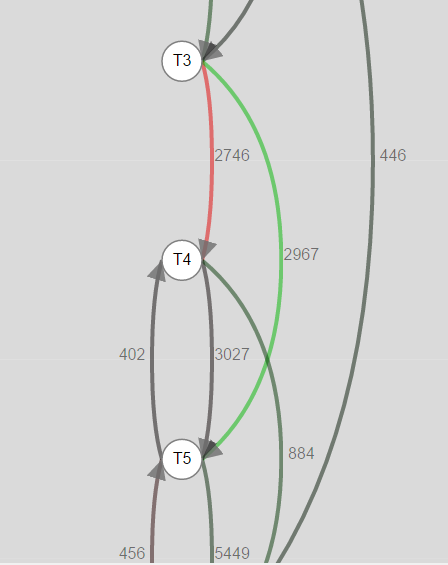
\includegraphics[width=0.45\linewidth]{images/PM_anomaly.PNG}
\caption{Аномалия в графе переходов}
\label{fig:processmap}
\end{figure}


\subsection{Хендлеры (способы рекомендации)}
\indent В этом параграфе будут перечислены функции-хендлеры, каждая из которых реализует свой способ рекомендаций. Хендлер принимает в качестве параметров пользователя, а также урок, на котором тот находится, если рекомендация контекстная. Хендлер возвращает для пользователя $j$ список уроков, в котором каждому уроку $i$ соответствует вес $weight_{ij} \in [0,1]$, чем он больше, тем лучше рекомендация:  $[(i, weight_{ij})]$. 

\\\indent Пусть мы хотим порекомендовать пользователю $j$ уроки по конкретному тегу, для которого доля пройденных пользователем уроков составляет $tag\_progress_j$. В случае, если по нему нет путей, все его уроки получают вес  $tw_{ij} =tag\_progress_j$. Если же путь есть, то для каждого урока этот вес делится на расстояние до ближайшего предшествующего в пути урока, пройденного пользователем $j$: $tw_{ij} = tag\_progress_j / dist_{ij}$. Таким образом реализуется идея, что пользователю может быть интересно проходить материалы, расположенные в пути недалеко от уже изученных им.

\begin{itemize}
    \item \textit{Уроки с интересными пользователю тегами} -- хендлер советует уроки, помеченные тегами, которые пользователь уже изучал. Для этого используется описанная выше рекомендация по тегам, вес урока $i$ для пользователя $j$ будет составлять $weight_{ij} = tw_{ij}$.
    \item \textit{Незаконченные уроки} -- советуются уроки, которые пользователь начинал и не закончил, с весом тем большим, чем большую часть урока пользователь прошел: $weight_{ij} = lesson\_progress_{ij}$, доля урока $i$, пройденного пользователем $j$. 
    \item \textit{Популярные уроки} -- хендлер не использует информацию о пользователе, а советует просто самые популярные за последнюю неделю уроки на платформе. Вес прямо пропорционален популярности: $weight_{ij} = 1 / n_i$, где $n_i$ -- номер урока $i$ в списке популярных уроков.
    \item \textit{Пути по урокам} -- используются пути, содержащие уроки, которые пользователь проходил, советуются уроки следом за пройденными, с весом тем меньшим, чем дальше урок от уже пройденных: $weight_{ij} = 1 / dist_{ij}$, где  $dist_{ij}$ -- расстояние от урока $i$ до ближайшего предшествующего в пути урока, пройденного пользователем $j$.
    \item \textit{Граф переходов по тегам} -- рекомендуются уроки с тегами, которые изучают после тегов, интересующих пользователя. Веса зависят от прогрессов пользователя по тегам, а также от относительных частот переходов между тегами. Пусть $freq$ -- частота перехода от тега, уроки которого пользователь изучал, к некоторому тегу $t$. Тогда для урока $i$, помеченного тегом $t$, вес рекомендации пользователю $j$ будет $weight_{ij} = freq \cdot tw_{ij}$. 
    \item \textit{Уроки по тегам от похожих пользователей} -- на основе интересующих пользователя тегов выявляются пользователи с похожими на его интересами, и рекомендуются уроки с тегами, которые они сами изучают. Пусть у текущего пользователя $j$ нашелся похожий на него пользователь $k$, причем мера схожести между ними -- $s$ (лежит между $0$ и $1$, чем она больше, тем более схожи пользователи). Тогда урок $i$, помеченный тегом, который изучал $k$, будут советоваться с весом $weight_{ij} = s \cdot tw_{ij}$. Этот хендлер реализует способ рекомендаций с помощью колаборативной фильтрации.
    \item \textit{Граф переходов по урокам} (только при контекстных рекомендациях) -- хендлер советует уроки, следующие за текущим в графе переходов, вес зависит от относительной частоты перехода между текущим уроком и советуемым. Если переход из текущего урока в урок $i$ совершается с относительной частотой $freq_i$, то  $weight_{ij} = freq_i$.
    \item \textit{Пути по урокам (только при контекстных рекомендациях)} -- советуются уроки, следующие за текущим в каких-либо путях, веса обратно пропорциональны расстоянию между уроками: $weight_{ij} = 1 / dist_{i}$, где $dist_i$ -- расстояние от урока $i$ до текущего урока.
    \item Если все предыдущие хендлеры в совокупности посоветовали меньше уроков, чем было нужно, в рекомендации добавляются случайные уроки, вес таких уроков равняется $0$.
\end{itemize}


\subsection{Оценка реакции пользователя}
\indent Чтобы понять, насколько успешна оказалась рекомендация, после ее показа фиксируется, перешел ли пользователь по ссылке, а также какую часть от урока пользователь прошел. В то же время у пользователя есть возможность узнать, почему урок был посоветован (варианты соответствуют хендлерам) и пометить рекомендацию как не интересную ему. Также мы располагаем сведениями о том, какую часть урока пользователь прошел (значение от $0$ до $1$).
\\\indent В результате каждой показанной рекомендации мы можем сопоставить некоторое число: $-1$ соответствует отказу от рекомендаций, $1$ -- переходу по ссылке без прохождения урока, $2$ -- переходу по ссылке и полному прохождению урока, значение от $1$ до $2$ -- неполному прохождению урока, а $0$ -- отсутствию реакции.


\subsection{Формирование выдачи}
\indent Итак, мы получили списки уроков от нескольких хендлеров, в которых каждому уроку сопоставлен вес от $0$ до $1$, чем больше, тем более удачной оценивает хендлер рекомендацию. Встает вопрос, как их лучше всего комбинировать
\\\indent Можно было бы просто для каждого урока сложить или перемножить веса хендлеров, которые его посоветовали. Но это означало бы, что мы полагаем разные хендлеры одинаково полезными, что, вообще говоря, может быть совсем не так. Хотелось бы оценить каждый хендлер коэффициентом полезности, используя при этом реакции пользователей на рекомендации. Таким требованиям удовлетворяет линейная регрессия.
\\\indent На рис.~\ref{fig:handlers_scheme} схематически изображен этот процесс. Регрессионная модель обучается с использованием накопленных данных о том, как рекомендации разных хендлеров были оценены пользователем. Исходя из этого модель формирует вектор весов для хендлеров, вес хендлера соответствует его полезности и влияет на его вклад в выдачу. Далее, когда требуется конкретная рекомендация, регрессионная модель для каждого урока комбинирует веса предложивших его хендлеров с использованием своего вектора весов для них, и выдает результирующий вес для каждого рекомендованого урока.

\begin{figure}[t]
\centering
\includegraphics[width=\linewidth]{images/handlers_scheme.png}
\caption{Использование линейной регрессии}
\label{fig:handlers_scheme}
\end{figure}

\indent Ниже представлено формальное описание регрессионной модели.

\subsubsection{Линейная регрессия}
\indent \textit Пусть у нас есть матрица $X = \{x_i^j\}_{i \in \{1, ..., n\} \\ j \in \{1, ..., d\}}$, $x_i\in\mathbb{R}^{d}$, строки которой $x_i = (x_i^1, ... x_i^d)$ называются \textit{наблюдениями}, а столбцы \textit{факторами}, и столбец значений \textit{целевой} или \textit{зависимой} переменной $y = \{y_i\}_{i=1}^n$. Регрессионная модель $y = f(X, b) + \epsilon$, где $b$ -- параметры модели, а $\epsilon$ -- случайная ошибка, называется \textit{линейной}, если зависимость целевой переменной от факторов является линейной, то есть $f(x, b) = b_0 + \sum_{i=1}^{d} b_i \cdot x_i$. Обычно для удобства $b_0$ (\textit{константу}) вносят под знак суммы, добавив в матрицу наблюдений столбец из единиц: $x_i^0 = 1$ для всех $i \in \{1, ..., n\}$. 
$$X = \left(\begin{array}{c}
      x_1 \\
      \vdots \\
      x_n
    \end{array}
  \right) 
  = 
  \begin{pmatrix} x_1^0 & x_1^1 & \cdots & x_1^d \\
                      x_2^0 & x_2^1 & \cdots & x_2^d \\
                      \vdots & \vdots & \ddots & \vdots \\
                      x_n^0 & x_n^1 & \cdots & x_n^d \end{pmatrix}
y = \left(\begin{array}{c}
      y_1 \\
      \vdots \\
      y_n
    \end{array}
  \right)
\beta = \left(\begin{array}{c}
      b_0 \\
      \vdots \\
      b_d
    \end{array}
  \right)
\epsilon = \left(\begin{array}{c}
      \epsilon_1 \\
      \vdots \\
      \epsilon_n
    \end{array}
  \right)$$
\\\indent Используя эти обозначения, линейную регрессионную модель можно выписать как $y = X \beta + \epsilon$. Решением этой задачи будем считать столбец $\hat\beta$, который минимизирует сумму квадратов отклонений предсказываемых значений от реальных, то есть $\displaystyle \hat\beta = {\rm arg}\min_{\beta\in\mathbb{R}^{d+1}} \sum_{i=1}^n (y_i - x_i \beta)^2$. Такой способ аппроксимации называется \textit{методом наименьших квадратов} (\textit{ordinary least squares}) и является наиболее широко применимым в контексте решения задачи линейной регрессии.
\\\indent В нашем случае мы можем рассматривать в качестве наблюдений, то есть строк матрицы $X$, рекомендованные уроки, в качестве факторов этих наблюдений веса, которые хендлеры назначили уроку, а в качестве значений целевой переменной -- оценку рекомендации пользователем.
\\\indent Таким образом, для уроков $i_1, \cdots, i_n$, посоветованных пользователям $j_1, \cdots, j_n$ соответственно, и для хендлеров $1, \cdots, 9$ матрица наблюдений $X$ и столбец значений целевой переменной (реакции пользователя) $y$ будут выглядеть следующим образом:
$$X =
  \begin{pmatrix} weight_{i_1 j_1}^1 & weight_{i_1 j_1}^2 & \cdots & weight_{i_1 j_1}^9 \\
                      \vdots & \vdots & \ddots & \vdots \\
                      weight_{i_n j_n}^1 & weight_{i_n j_n}^2 & \cdots & weight_{i_n j_n}^9 \end{pmatrix}
y = \left(\begin{array}{c}
      r_{j_1} \\
      \vdots \\
      r_{j_n}
    \end{array}
  \right)$$         
 
\\\indent Вектор $\hat\beta$, который дает минимальную ошибку предсказания реакции пользователя, содержит индивидуальный вес для каждого из хендлеров, на который нужно домножать его рекомендации. Если вес какого-то из хендлеров относительно большой, значит, этот хендлер вносит положительный вклад в рекомендации, и наоборот. 
\\\indent Для работы рекомендательной системы регрессионная модель будет на регулярной основе обучаться на данных о реакции пользователей на рекомендации. Мы будем использовать библиотеку SciPy\cite{scipy} для решения этой задачи и нахождения столбца $\hat\beta$. В этой библиотеке уже реализовано решение задачи линейной регрессии.

\paragraph{Регуляризация}
\indent После первичной реализации рекомендательной системы с линейной регрессией, которая находила столбец весов для хендлеров $\hat\beta$, минимизирующий квадрат отклонений реальной реакции пользователя от предсказанной ($\displaystyle \hat\beta = {\rm arg}\min_{\beta\in\mathbb{R}^{d+1}} \sum_{i=1}^n (y_i - x_i \beta)^2$), стало заметно, что постепенно вес одного хендлера неограниченно возрастает, в то время как остальные уменьшаются, что в итоге привело к формированию выдачи практически только из результатов этого хендлера. Такой эффект называется \textit{положительной обратной связью}, и характеризуется тем, что отклонение в результатах работы системы влияет на ее дальнейшую работу, причем чем дальше, тем больше результаты сдвигаются в сторону этого отклонения.
\\\indent Помимо этого, так как хендлеры могут предлагать очень схожые рекомендации, в наших данных также может присутствовать проблема \textit{мультиколлинеарности} факторов, что влечет за собой слабую обособленность матрицы $X$ и, как следствие, нестабильность решения.
\\\indent В результате мы получаем решение, которое дает маленькую ошибку на данных, на которых оно обучается, и большую на реальных данных. Эта ситуация называется \textit{переобучением} (\textit{overfitting}) модели.
\\\indent В качестве решения проблемы переобучения можно рассмотреть регуляризацию. Согласно книге \textit{The Elements of Statistical Learning}\cite{hastie2001elements}, основные способы регуляризации -- это \textit{лассо} (LASSO, least absolute shrinkage and selection operator \cite{lasso}) и \textit{гребневая регрессия} (регуляризация Тихонова, ridge regression \cite{ridge}). Оба этих метода меняют выражение, которое мы минимизируем в процессе поиска решения регрессии, добавляя к нему штраф на норму вектора $\beta$. 
\\\indent В случае лассо-регуляризации используется $l_1$-норма и решение находится как $$\displaystyle \hat\beta = {\rm arg}\min_{\beta\in\mathbb{R}^{d+1}}( \sum_{i=1}^n (y_i - x_i \beta)^2 + \lambda ||\beta||_1).$$
\\\indent В случае же гребневой регрессии используется $l_2$-норма и решение выглядит как $$\displaystyle \hat\beta = {\rm arg}\min_{\beta\in\mathbb{R}^{d+1}}( \sum_{i=1}^n (y_i - x_i \beta)^2 + \lambda ||\beta||_2).$$ В обоих случаях параметр $\lambda$ подбирается в процессе оптимизации.
\\\indent Использование регуляризации методом лассо уменьшает все $\beta_i$, а те, что и так были относительно небольшими, становятся равны нулю. Таким образом, метод лассо хорошо подходит для выбора значащих факторов (feature selection).  
\\\indent Метод гребневой регрессии также уменьшает веса факторов, но при этом никогда не сводит их к нулю, если только не $\lambda = \infty$.
\\\indent Согласно работе \cite{Ng04featureselection} лассо-регуляризация работает лучше гребневой в ситуации, когда количество факторов значительно превосходит число обучающих наблюдений. В обратной же ситуации более уместна гребневая регрессия. Соответственно, для нашего случая лучше подходит именно она. Её реализация также присутствует в библиотеке SciPy.



\section{Адаптивная рекомендательная система}
\indent В рамках классического офлайн-обучения важную роль играет постоянный контроль преподавателем уровня знаний обучающегося, который позволяет своевременно скорректировать программу, дать дополнительные задачи для закрепления плохо усвоенного материала, а также подсказать ресурсы для восполнения пробелов в знаниях. В контексте массового онлайн-обучения такой возможности нет, так как студентов может быть от нескольких сотен до десятков тысяч. Вследствие этого важной характеристикой рекомендательной системы является \textit{адаптивность}, то есть способность системы подстраиваться под уровень знаний конкретного пользователя, учитывая, что этот уровень к тому же меняется в процессе обучения.
\\\indent Одной из первых задач в этой области было \textit{компьютерное адаптивное тестирование} (\textit{Computerized Adaptive Testing, CAT})\cite{CAT}. Суть этой задачи в том, чтобы оценивать знания в некоторой области с помощью теста, но не одного для всех учащихся, а индивидуальных, составляющихся динамически в процессе прохождения теста из имеющегося набора задач, чтобы сократить длину теста, не заставляя пользователя решать слишком простые или сложные для него задачи. Вопросы теста оцениваются различными параметрами (в основном используются сложность и дискриминативность, то есть способность задачи отделить в рамках рассматриваемой области слабых учащихся от сильных), информация о знаниях пользователя также комбинируется в некоторый общий параметр, и на каждом шаге пользователю предлагается такая задача, которая будет примерно той же сложности, какого уровня знания пользователя в данный момент, и при этом максимальной дискриминативности. Это позволяет сократить количество вопросов в тесте, не теряя при этом качество оценки. В качестве примера использования такого подхода будет рассмотрена система адаптивных тренировок по математике для учеников начальных классов MathsGarden\cite{mathsgarden}.
\\\indent Ещё одной важной чертой адаптивной системы является возможность использовать связи между контентом, подсказывать пользователю, что ему изучить, чтобы лучше понимать текущий материал. В качестве примера такой системы можно привести платформу Knewton\cite{knewton_paper}, которая предоставляет функциональность для изучения любого материала в адаптивном режиме. В числе прочего для этого активно используется \textit{граф знаний}, описывающий связи и зависимости между темами материала. С использованием этого графа ученику, не справляющемуся с темой, можно подсказать материалы по теме, предшествующей текущей в графе знаний, например, для понимания алгоритма Евклида нужно сперва разобраться с тем, что такое наибольший общий делитель. Такой подход требует обширной ручной разметки материала.

\subsection{MathsGarden}
\indent Сервис адаптивных математических тренировок для учащихся младшей школы MathsGarden\cite{mathsgarden} был разработан в Нидерландах в 2010 году. В качестве основы была взята обычная методика компьютерного адаптивного тестирования: из набора доступных задач выбирается такая, которая лучшим образом подходит пользователю по сложности в данный момент, результат решения анализируется, информация об уровне пользователя обновляется, процесс итеративно повторяется, пока не будет выполнен терминирующий критерий (например, ограничение по времени или требуемая уверенность в оценке студента). 
\\\indent Модель, использовавшаяся в этом сервисе, была использована и в нашей рекомендательной системе. Нижу я опишу эту модель подробнее.
\subsubsection{Выбор наиболее подходящей задачи}
\indent Для определения подходящей пользователю задачи сегодня чаще всего используется стохастическая теория тестов (\textit{IRT, Item Response Theory})\cite{CAT}, основополагающей чертой которой является предположение, что вероятность решения пользователем задачи суть функция от параметров пользователя и задачи. Она получила широкое распространение на фоне классической теории тестирования, так как в отличие от неё допускала различие в сложности задач. В общем случае используется логистическая функция трёх параметров (\textit{three parameter logistic function, 3PL function}): вероятность пользователю с уровнем знаний $\theta$ решить задачу $i$ выражается как $p_i(\theta) = c_i + \frac{1 - c_i}{1 + e^{-a_i(\theta - b_i)}}$, где $b_i$ -- сложность задачи, $a_i$ -- параметр дискриминативности, а $c_i$ -- шанс случайно угадать ответ на задачу \cite{IRTapplications}. При этом не обязательно использовать все параметры, в частности, создатели MathsGarden используют лишь один из них, сложность задачи, что дает однопараметрическую (1PL) модель, также известную как модель Раша\cite{rasch_model}.
\\\indent Существуют математическое доказательство того, что наиболее быстро и точно провести адаптивное тестирование можно при выборе таких задач, сложность которых равняется текущей оценке знаний студента. При таком выборе средний шанс решить задачу -- 50\%, что в целом демотивирует студента\cite{ericsson2006influence}. Создатели MathsGarden, основываясь на исследовании своих коллег\cite{time_scoring_rules}, сделали средний шанс около 75\%, что ухудшило качество, но затем привнесли в оценку исхода <<игры>>, то есть решения задачи, информацию о затраченном на решение времени. После этого качество оценки вернулось к исходным показателям\cite{mathsgarden}.


\subsubsection{Рейтинг Эло}
\indent Одной из основных проблем при использовании CAT является необходимость заранее разметить задачи параметрами, использующимися в психометрической модели, определяющей наиболее подходящий вопрос. Чтобы избежать ручной разметки, исследователи совместили адаптивное тестирование с динамическим вычислением сложности задач и способностей пользователя, используя для этого модификацию системы рейтингования в шахматах, разработанную Арпадом Эло в 1978 \cite{elo1978rating}. Суть системы в том, что перед каждой игрой её результат предсказывается, а после завершения игры рейтинги игроков пересчитываются с учетом разницы между предсказанным счётом и реальным. В качестве игроков рассматриваются учащийся и задача, которую он решает, в качестве их рейтингов выступают соответственно оценки знаний студента и сложности задачи. В классической шахматной системе результат игры между игроками $j$ и $k$ для первого из них $S_j \in \{0, 0.5, 1\}$ (проигрыш, ничья и выигрыш соответственно), а ожидаемый результат вычисляется как $E(S_j) = \frac{1}{1 + 10 ^ {(\theta_j - \theta_k) / 400}}$, где $\theta_j$ и $\theta_k$ -- рейтинги игроков. Обновлённый рейтинг игрока $j$ в таком случае вычисляется как $\hat{\theta_j} = \theta_j + K(S_j - E(S_j))$. Параметр $K$ определяет то, как сильно расхождение между ожидаемым результатом и реальным влияет на изменение рейтинга. В классической модели $K$ -- константа (точнее, несколько констант для разных категорий игроков), но Марк Гликман предложил сделать это значение зависимым от конкретной ситуации\cite{glickman95} для большей гибкости системы.
\\\indent Для этого помимо сведений об уровне знаний и сложности вводятся также параметры, описывающие нашу неуверенность в текущей оценке ситуации. Это нужно для того, чтобы поведение системы варьировалось: в случае нового игрока, про которого мы почти ничего не знаем, его рейтинг мог быстро меняться с каждой игрой, а в случае профессионала, сыгравшего на нашей памяти уже сотни игр, чей рейтинг посчитан на основании большого объема данных о его уровне, один проигрыш не повлёк за собой значительного падения его рейтинга. Параметры неопределенности пересчитываются в зависимости от частоты решений и давности последнего из них. Такой параметр есть как у пользователя, так и у задачи.

\subsubsection{Механика работы}

\begin{figure}[t]
  \centering
  \subfloat[начальный экран]{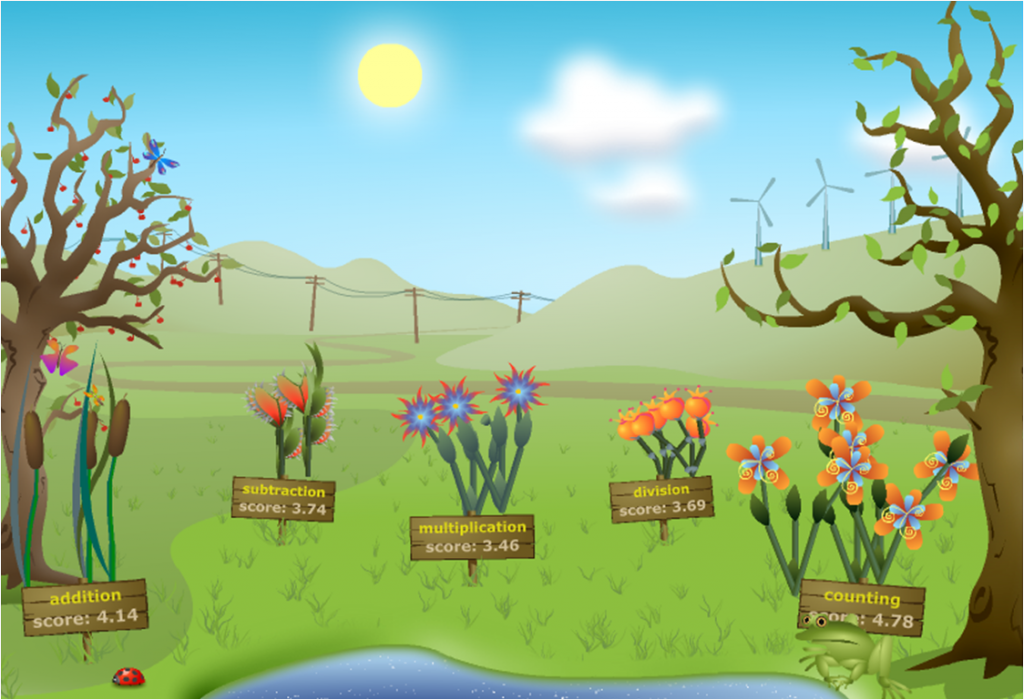
\includegraphics[width=0.4\textwidth]{images/mathsgarden.png} \label{fig_mathsgarden1}}
  \hfill
  \subfloat[решение задачи]{
\includegraphics[width=0.5\textwidth]{images/mathsgarden_quiz.png} \label{fig_mathsgarden2}}
  \caption{Интерфейс сервиса MathsGarden}
  
\end{figure}

\indent На начальной странице ресурса (рис.~\ref{fig_mathsgarden1}) учащемуся предлагается выбрать одну из областей для тренировки (сложение, вычитание и прочие). Области изображены в виде цветков, под каждым из которых написан текущий уровень ученика в этой области. После выбора темы пользователю предлагается несколько задач (рис.~\ref{fig_mathsgarden2}), на каждую из которых отводится $20$ секунд. В зависимости от правильности ответа и времени, потраченного на решение, пользователь либо получает, либо лишается нескольких монет.
\\\indent Пользователю предлагаются задачи, вероятность решить которые в данный момент для него ближе всего к 75\%. После решения задачи вычисляется результат, зависящий от правильности ответа и от времени, потраченного на решение. Отклонение этого результата от предсказанного влияет на изменения значений сложности задачи и уровня пользователя.

\subsubsection{Результаты работы}
\indent Сервис MathGarden использовался приблизительно 150 школами в течение года, после чего накопленные данные были проанализированы. Основные результаты следующие:
\begin{itemize}
    \item полученные оценки знаний учеников коррелируют с их результатами в общем рейтинге учеников CITO. В разных темах (сложение, вычитание и прочие) корреляция составила от $0.78$ до $0.84$;
    \item надёжность оценки сложности анализировалась в числе прочего через проверку корреляции сложности зеркальных задач ($4+7$ и $7+4$ должны иметь почти одинаковую сложность), значения которой оказались между $0.88$ и $0.98$ среди разных тем;
    \item также был проведен анализ устойчивости сложности со временем. Корреляция оказалась не менее $0.95$ между срезом на $44$ неделе и каждой из последующих $32$ недель.
\end{itemize}


\subsection{Адаптивность в stepic.org}
Для рекомендательной системы на stepic.org было решено добавить хендлер, который будет в рамках одного курса советовать пользователю уроки, подходящие ему в данный момент по сложности. Для вычисления сложности была использована модель, разработанная в MathsGarden. Для задач были добавлены параметры сложности ($\beta_i$) и неопределенности оценки ($U_i$), а для каждого пользователя и курса, который он проходит, был заведен параметр его уровня в этой теме ($\theta_j$) и также неопределенность оценки ($U_j$). Формулы, приведённые ниже, взяты из описания сервиса MathsGarden\cite{mathsgarden}, с небольшими изменениями для использования в нашей системе.
\\\indent Для оценки результата решения задачи $i$ пользователем $j$ используется следующая формула: $S_{ij} = (2 x_{ij} - 1)(1 - t_{ij} / d_i) $, где $x_{ij} = 1$, если ответ верный, иначе $0$, $t_{ij}$ -- минимальное значение из времени, потраченного на решение, и $d_i$, а $d_i$ -- время, за которое в среднем пользователи решают эту задачу (в MathsGarden $d_i$ всегда $20$ секунд). Предполагаемые результаты решения вычисляются как $E(S_{ij}) =  \frac{e^{2 (\theta_j - \beta_i)} + 1}{e^{2 (\theta_j - \beta_i)} - 1} - \frac{1}{\theta_j - \beta_i}$, где $\beta_i$ -- сложность задачи, $\theta_j$ -- уровень пользователя\cite{time_scoring_rules}. Формулы учитывают время, причем чем меньше времени было потрачено, тем больше вознаграждение или штраф. Учёт времени в подсчёте результата решения позволяет без потери качества предлагать пользователю задачи с шансом решить их больше 50\%, что повышает мотивацию\cite{mathsgarden}\cite{ericsson2006influence}.
\\\indent Далее оценка знаний студента и сложности задачи обновляется по формулам $\hat{\theta_j} = \theta_j + K_j(S_{ij} - E(S_{ij}))$ и  $\hat{\beta_i} = \beta_i + K_i(E(S_{ij}) - S_{ij})$ соответственно. Коэффициенты $K_i$ и $K_j$ влияют на то, как сильно различия между предсказанным исходом и реальным изменят рейтинги. Они вычисляются по формулам  $K_j = K(1 + K_+ U_j - K_- U_i)$, $K_i = K(1 + K_+ U_i - K_- U_j)$, где $U_i$ и $U_j$ -- параметры студента и задачи соответственно, характеризующие нашу неуверенность в их оценках, $K = 0.0075$, $K_+ = 4$ и $K_- = 0.5$\cite{mathsgarden}. Использование коэффициентов, зависящих от конкретных пользователей и задач, делает систему более гибкой\cite{glickman95}.
\\\indent Параметры неопределенности $U$ зависят от частоты и давности решений, $0 \le U \le 1$. Пересчитываются их значения при каждом решении для пользователя и для задачи следующим образом: $\hat{U} = U - \frac{1}{40} + \frac{1}{30} D$, при каждом пересчете (использовании) неопределенность уменьшается на $\frac{1}{40}$, со временем ($D$ -- число дней без использования задачи / без практики пользователя) увеличивается. Изначально $U$ равняется единице.
\\\indent Для решения пользователю предлагаются задачи, вероятность решить которые в данный момент ближе всего к 75\%.

% TODO: нарисовать графиков логистических кривых для примера
% оформить формулы более структурировано



\section{Анализ результатов}
\indent Для анализа работы получившейся рекомендательной системы целесообразно выбрать интуитивно понятные метрики. Рассмотрим основные классы метрик, применяющихся для оценки рекомендательных систем\cite{rec_sys_handbook:evaluation}:
\begin{itemize}
    \item \textit{Предпочтение пользователей}: какую из множества систем пользователи используют наиболее охотно. Используется в случае, когда есть возможность провести сравнение, предложив различные системы нескольким группам пользователей. Метрики этого класса считаются для всех интересующих систем, после чего сравниваются.
    \item \textit{Точность предсказания}: применяется в случае, если система предсказывает отношение пользователя к объектам (например, выставляемые ими рейтинги) или вероятность использования пользователем контента. К этому классу также относятся метрики, оценивающие качество ранжирования списка рекомендаций.
    \item \textit{Покрытие}: какую часть из интересных пользователю объектов система смогла предсказать. Обычно затрудняется отсутствием полной информации о интересах пользователя.
    \item \textit{Надежность}: можно ли в целом доверять рекомендациям. Позволяет отделить систему с в среднем неплохими рекомендациями от такой, в которой на пару отличных рекомендаций будет приходиться десяток совершенно не уместных.
    \item Прочие метрики, такие как доверие пользователя системе, новизна и разнообразие предлагаемых рекомендаций и прочие.
\end{itemize}

\indent Также возможны разные режимы оценки рекомендаций:
\begin{itemize}
    \item \textit{офлайн-оценка}: предварительно набирается информация о пользователях, симулируется работа системы, результаты оцениваются исходя из тех же данных;
    \item \textit{искусственные исследования}: специально отобранной группе пользователей предлагается опросник, который им нужно заполнить в процессе использования системы, также исследуются накопленные в процессе данные о работе системы;
    \item \textit{онлайн-оценка}: рекомендательная система испытывается в <<боевых условиях>>.
\end{itemize}

\indent В этой работе будут использоваться оценки, посчитанные на основе реальных данных об использовании пользователями системы в нормальном режиме. Исследованы данные о простых рекомендациях пользователю на основе информации о нем, о рекомендациях в конце урока (контекстные рекомендации) и об адаптивных рекомендациях. 
\indent В первых двух случаях рекомендации показываются пользователю списком уроков, которые могут его заинтересовать. В случае простых рекомендаций в этом списке двадцать уроков, в случае контекстных -- пять. Адаптивные рекомендации представляют собой один урок, который по подсчетам системы подходит пользователю в данный момент лучше всего. Будем называть каждый конкретный случай подсчета рекомендаций для пользователя \textit{рекомендательной сессией}.

\subsection{Простые рекомендации}
\indent Рекомендации для пользователя показываются списком из $20$ уроков. У пользователя есть возможность узнать, почему ему был посоветован этот урок (причины берутся из хендлеров, предложивших его), а также отказаться от рекомендации конкретного урока, нажав на соответствующую кнопку возле этой рекомендации. 
\\\indent Для оценки будут использоваться следующие метрики:

\begin{itemize}
    \item Процент сессий, в которых был совершен хотя бы один переход по ссылке или отказ от рекомендации. К сожалению, так как рекомендации показываются на главной странице, где не многие их действительно видят, этот процент будет невелик. Дальнейшие метрики будут рассматриваться только для сессий, на которые была получена какая-то реакция, положительная (переход по ссылке) или отрицательная (отказ от рекомендации);
    \item Среднее число переходов по ссылке в сессии;
    \item Какую часть урока в среднем проходят пользователи после перехода по ссылке;
    \item Сколько совершено отказов от рекомендаций.
\end{itemize}

\indent Были исследованы данные о работе системы за четыре месяца. Результаты представлены в таблице \ref{tabular:table_usual}.

\begin{table}[h]
    \caption{Результаты для простых рекомендаций}
    \label{tabular:table_usual}
    
    \begin{center}
    \begin{tabular}{ c | r }
      \hline
      Метрика & Значение \\
      \hline	
      \hline
      Число сессий & 381868 \\
      Число сессий с реакцией & 18066 \\
      Процент сессий с реакцией &  4.7\% \\
      Число открытых рекомендаций (из 20) & 1.6 \\
      Пройденная часть урока & 0.52 \\
      Число отказов от рекомендации & 184 \\\hline
    \end{tabular}
    \end{center}
\end{table}

\\\indent На рис.~\ref{fig:usual_distibutions} представлены распределения числа открытых рекомендаций и пройденной части урока.

\begin{figure}[h]
  \centering
  \subfloat[открыто ссылок]{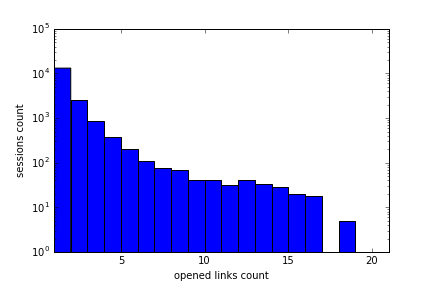
\includegraphics[width=0.5\textwidth]{images/home_page_opened_links_number_hist.png}}
  \hfill
  \subfloat[доли решения]{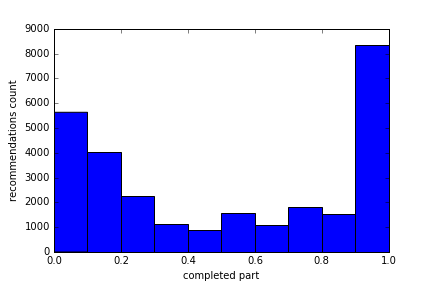
\includegraphics[width=0.5\textwidth]{images/home_page_completed_part_hist.png}}
    \caption{Распределения для простых рекомендаций}
    \label{fig:usual_distibutions}
\end{figure}


\subsection{Контекстные рекомендации}
\indent В случае, если урок, пройденный пользователем, не включен ни в какой курс, то есть не имеет явного следующего за ним урока, пользователю предлагаются рекомендации, сделанные на основе информации о нем и о текущем уроке. В данном случае пользователь наверняка видел рекомендации, что прямо отражается на проценте рекомендательных сессий с реакцией.
\\\indent В таблице \ref{tabular:table_context} также отражены результаты за четыре месяца.

\begin{table}[h]
    \caption{Результаты для контекстных рекомендаций}
    \label{tabular:table_context}
    
    \begin{center}
    \begin{tabular}{ c | r }
      \hline
      Метрика & Значение \\
      \hline	
      \hline
      Число сессий & 26995 \\
      Число сессий с реакцией & 15125 \\
      Процент сессий с реакцией &  56\% \\
      Число открытых рекомендаций (из 5) & 1.48 \\
      Пройденная часть урока & 0.5 \\
      Число отказов от рекомендации & 0 \\
      \hline  
    \end{tabular}
    \end{center}
\end{table}


\\\indent На рис.~\ref{fig:context_distibutions} представлены распределения числа открытых рекомендаций и пройденной части урока.

\begin{figure}[h]
  \centering
  \subfloat[открыто ссылок]{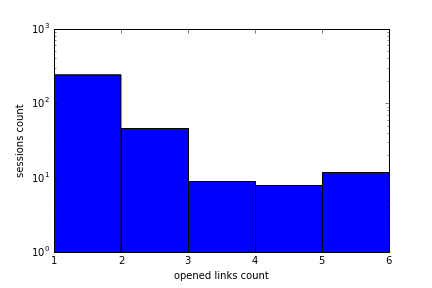
\includegraphics[width=0.5\textwidth]{images/context_opened_links_number_hist.png}}
  \hfill
  \subfloat[доли решения]{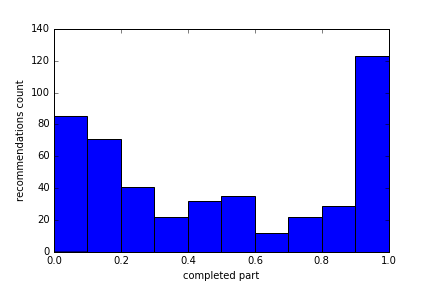
\includegraphics[width=0.5\textwidth]{images/context_completed_part_hist.png}}
    \caption{Распределения для контекстных рекомендаций}
    \label{fig:context_distibutions}
\end{figure}

\subsection{Адаптивные рекомендации}
\indent Для оценки качества адаптивных рекомендаций использовались данные, накопленные за две недели работы. Эти две недели пользователям было предложено проходить в адаптивном режиме курс-тренажер по языку программирования Python. 
\\\indent Пользователь получал рекомендованный урок, после чего он мог пометить его слишком сложным, слишком простым или решить его. Его действия влияли на то, какой уровень знаний ($skill$) система присваивала ему, и какую сложность ($\mathit{difficulty}$) -- задаче. При этом для каждой рекомендации рассчитывалось предсказание исхода ($1$ -- решил, $0$ -- не решил). Это позволяет вычислить средне-квадратичную ошибку (mean square error, MSE) предсказания: $$MSE = \sum_{k=0}^{N}(predicted_k - real_k)^2,$$ где $N$ -- число примеров, $predicted_k$ и $real_k$ -- предсказанный и реальный результаты для $k$-го примера.
\\\indent В таблице \ref{tabular:table_adaptive} представлены основные метрики работы системы.


\begin{table}[h]
    \caption{Результаты для адаптивных рекомендаций}
    \label{tabular:table_adaptive}
    \begin{center}
    \begin{tabular}{ c | r }
      \hline
      Метрика & Значение \\
      \hline
      \hline
      Число сессий & 1511 \\
      Число пользователей & 246 \\
      Реакций <<решено>> & 1329 \\
      Реакций <<слишком просто>> & 95 \\ 
      Реакций <<слишком сложно>> & 87 \\
      MSE предсказания исхода & 0.22 \\
     \hline  
    \end{tabular}
    \end{center}
\end{table}

\\\indent Также было исследовано, действительно ли ошибка предсказания для конкретного пользователя или задачи уменьшается со временем. Для этого ошибки были усреднены по пользователям (рис.~\ref{fig:adapt1}) и по задачам (рис.~\ref{fig:adapt2}). На получившихся графиках наблюдается явное, хоть и не равномерное, убывание ошибки.


\begin{figure}[h]
  \centering
  \subfloat[пересчет знаний пользователя]{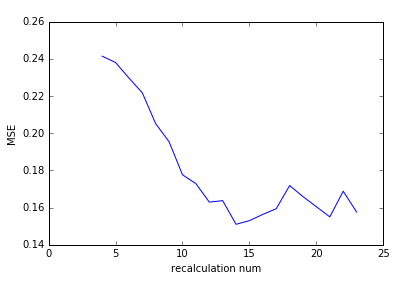
\includegraphics[width=0.45\textwidth]{images/mse_user_skill.png}
    \label{fig:adapt1}}
  \hfill
  \subfloat[пересчет сложности задачи]{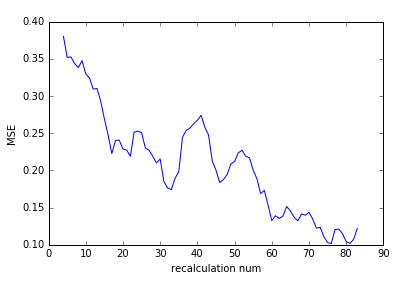
\includegraphics[width=0.45\textwidth]{images/mse_quiz_difficulty.png}
  \label{fig:adapt2}}
    \caption{Изменение ошибки предсказания при пересчете}
    \label{fig:adaptive_errors}
\end{figure}



\section{Заключение}
\indent В рамках работы была реализована рекомендательная система для образовательного контента, которая теперь используется на платформе \textit{stepic.org}. Эта система совмещает в себе фильтрацию контента и коллаборативную фильтрацию, а также имеет возможность прохождения материала в адаптивном режиме, по индивидуальному для каждого учащегося пути. 
\\\indent Структура системы позволяет дополнять ее новыми способами рекомендации, причем значимость каждого способа и его вклад в итоговые рекомендации будет определяться системой автоматически на основе реакции пользователей.
\\\indent Также система предоставляет возможность получать рекомендации в разных ситуациях: как просто при входе на сайт, на домашней странице, так и в процессе обучения, сразу после прохождения урока. Помимо этого имеются также адаптивные рекомендации, подстраивающиеся под уровень знаний конкретного пользователя.
\\\indent В качестве дальнейших путей развития системы можно указать, во-первых, создание новых правил фильтрации контента исходя из нужд пользователей, во-вторых, совершенствование рекомендательной системы: используя ручную разметку контента можно при рекомендациях использовать изученные и не изученные пользователем темы, предлагать пройти ему что-то, знаний о чем ему не хватает для изучения интересного ему материала. Также возможна работа над проблемой <<холодного старта>>, ситуации, когда про пользователя и про материалы нет достаточного объема накопленных данных, что мешает с уверенностью давать рекомендации.



% ВОПРОСЫ
% 1. оформление: всякие курсивы, определки и прочее
% 2. код: нужен ли и в каком количестве?
% 3. общая структура, опять две части
% 4. надо evaluation!!






% цитата \cite{wiki:lcd}
% ссылка на label (\ref{лопиталь})
% ссылка на рисунок (рис.~\ref{разрыв_функции})


% У заключения нет номера главы
%\section*{Заключение}


\setmonofont[Mapping=tex-text]{CMU Typewriter Text}
\bibliographystyle{ugost2008ls}
\bibliography{diploma.bib}


\end{document}
